\chapter{Advanced Control}
\section{Introduction}
Cascade control is a type of closed-loop control with two or more control loops.

The actuator + the process can usually be modeled as different sub-systems connected to each other, so that there is one or more intermediate variables available for measurement.

Concept: controlling intermediate variables before their alterations by disturbances affect the output.

Result: cascade control minimizes the effect of disturbances in the inner loop (not so good for distrubances in the outer loop or for set point variations)

The objective of cascade control is to improve the dynamic response of a process by designing internal control loops according to identificable dynamics of sub-systems.

The tuning methods for the controllers are the ones studied in the basic control section.

\section{Cascade Control Design Methodology}
As mentioned in the intoruction, for cascade control, in addition to the controlled variable, one or more intermediate variables are fed back, giving rise to the appearance of nested loops in which the reference of an internal controller comes from the output of the controller immediately outside. The following figure shows the block diagram of a two-level cascade control, in which variable $y_2$ is fed back, in addition to the output.

\begin{figure}[H]
    \centering
    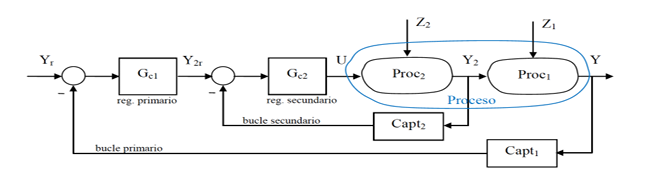
\includegraphics[width = 0.5 \textwidth]{Imagenes/4 - Cascade Control.png}
\end{figure}

Cascade control should only be designed if BRC does not provide satisfactory results. The key step is selecting the secondary variable to feed back.

\begin{itemize}
    \item It should be a variable that can be measured.
    \item It must indicate the occurence of an important distrubance
    \item There must be a causal relationship between the manipulated and secondary variables.
    \item The secondary variable dynamics must be faster than the primary variable dynamics.
\end{itemize}

\begin{enumerate}
    \item Identify the FOPDT functions of each subsystem by:
    \begin{itemize}
        \item Applying the studied methods, e.g. identification by the 63\% - tangent
        \item If applicable, applying the Fast-Slow method reduction.
    \end{itemize}
    \item After determination of the FOPDT functions of the processes, design the PID/PI controllers.
    \begin{enumerate}
        \item Tune the inner controller, based on the model of this part of the process. A PI controller is usually enough.
        \item Tune the outer controller, based on the model of the inner loop and the part of the process outside it. The inner loop model has no steady error and is usually very fast compared to the other part of the model.
    \end{enumerate}
    \item Compare the results with a basic control and decide the most suitable control strategy.
\end{enumerate}

\section{Feed forward control}
The purpose of feed-forward control is to cancel or at least reduce the effect of external disturbances on the system. In general it is not possible to completely cancel a disturbance, but when this perturbation occurs, at least its static component can usually be eliminated.

The objective of $G_{CA} (s)$ controller design is to eliminate the effect of distrubance $G_D (s)$.

\[ \frac{Y(s)}{D(s)} = 0 \rightarrow G_{CA} (s) = - \frac{G_D (s)}{G_P (s) G_S (s)} \]

The theoretical t.f. that fully eliminates the disturbance effect is not always feasible.
\begin{enumerate}
    \item $t_m$ in $G_{CA}(s)$ is not feasible when $t_{md} < (t_{mp} + t_{ms})$
    \item When the number of zeros($G_{CA} (s)$) > number of poles($G_{CA}(s)$)
\end{enumerate}

\section{Large delay systems: Smith's Predictor}

In previous sections we have studied the $rm= \frac{t_m}{t_p}$ coefficient, which defines the application ranges for ZN open-loop controllers $0.1 < r < 0.9$ and for the AMIGO controllers $0.25 < r < 3.0$.

Regarding the upper limit for the AMIGO controller, the upper limits can be defined approximately as a function of the relative delay $\tau$:
\[ \tau = \frac{T_t}{T_t + t_p} \]

For PID controllers: For values higher thatn 0.5 of the relative delay $\tau$, the PID control is comparable to PI. Hence, for slightly higher values, $\tau > 0.5$, a PI controller may be sufficient, although the designer should verify this properly, through simulations and select the best solution, PID or PI.

In any case, the upper bound is not easy to define and there are numerous research studying variations on PID controllers and the use of advanced techniques such as generic algorithms, etc.

Based on the above, if the controller design is in the upper limits (in this course we accept up to $r < 3.0$), we must simulate the behavior of the AMIGO controller vs. a controller for larga delays such as the Smith's Predictos and select the best option.

\subsection{Preliminaries}
Currently, there is a growing interest in time-delay plant control strategies, because time delay constitutes a very common phenomenon in the dynamic behavior of practically all industrial plants, process units, ecological, agricultural, biotechnological systems, etc.

Time delay is a phenomenon that originates due to the temporal displacement between two or more variables of a plant which can be generated, for example, by the time needed to transpor mass, energy or information. The time delay represents a significant limitation in control systems and must be considered, both in the analysis stages, as in the design controllers.

The design of appropriate controllers for plants with dominant time delay requires a grat effort, because if the disturbances are not detected in time, the control action, which depends on the timely measurement, does not occur at the right time, and takes time to take effect on the dynamic behavior of the plant. A delayed response of the plant to the control signal can cause a reaction of the controller that does not correspond to the required one, which can lead to loss of stability of the control system.

\subsection{Smith's Predictos (SP)}
The Smith's Predictor (SP) was proposed in 1957 by the American Otto Smith. It is undoubtedly the most widely used dead time compensator in the control of the time-delayed plants due to its high effectiveness and simple implementation.

This SP structure cannot be used in plants with integrators or in unstable plants, and it may also present a bad behavior for disturbance rejection.

Original idea: ``Take'' the delay out of the plant and design the controller for an internal $G_m(s)$ model with ``perfect'' prediction.

\subsubsection{Smith Predictor: add the actual error compared to the predicted output.}

\begin{figure}[H]
    \centering
    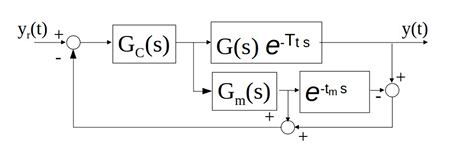
\includegraphics[width = 0.5 \textwidth]{Imagenes/4 - Smiths Predictor.png}
\end{figure}

Original idea: ``Take'' the delay out of the plant and design the controller for an internal model $G_m(s)$ with ``perfect'' prediction. Error feedback corrects the imperfections of the fast model $G_m(s) e ^{\tau s}$